\documentclass[10pt,a4paper]{article}
\usepackage[margin=20mm]{geometry}
\usepackage{amsmath,amssymb,graphicx,booktabs,longtable,microtype}
\usepackage[colorlinks=true,allcolors=blue]{hyperref}
\hypersetup{pdftitle={Supplementary methods, verification, and reproducibility: three-microphone azimuth estimation},pdfauthor={Aneesh Arnav Chikkala},pdfsubject={Supplement to a preprint for author review}}
\usepackage{fancyhdr}
\graphicspath{{../figures/}}
\pagestyle{fancy}\fancyhf{}\fancyhead[L]{\small Direction A: supplementary methods and checks}\fancyhead[R]{\small Author-review preprint}\fancyfoot[C]{\thepage}
\setlength{\headheight}{14pt}
\title{Supplementary methods, verification, and reproducibility\\\large Three-microphone azimuth estimation}
\author{Aneesh Arnav Chikkala}
\date{8 September 2026}
\begin{document}\maketitle
\noindent This supplement accompanies the server-neutral preprint. It records numerical corrections, the scope of the analytical bound, complete comparison definitions, and access to the retained frame results. It is not an independent peer-review report. Author confirmation of conflicts and approval of public release remain pending.

\section{Model definition and response support}
The image model uses the direct $1/(4\pi r)$ pressure amplitude, a fixed speed of sound 343 m/s, and products of real wall reflection coefficients. The production image coordinates are $2n_aL_a+(1-2p_a)s_a$, with low/high counts $|n_a-p_a|$ and $|n_a|$. All eight parity combinations are included. Source and microphone coordinates are strictly interior to the room. Direct arrivals remain later than the fractional kernel's head support, avoiding response truncation at time zero.

For the final campaign, nominal image extent is 76, path-duration cutoff is 1.2 s, propagation grid oversampling is 32, and the Kaiser-sinc decimation half-width is 32 acquisition samples. A response has 57,634 samples; the 59,682-sample prehistory includes the response support and an additional frame for acquisition-filter settling. The acquisition filter is causal: SciPy Butterworth prototype order four produces four second-order sections, hence total bandpass order eight. The frozen protocol uses the shorter prototype-order wording; this clarification does not change any generated signal. Source and noise histories are generated before cropping, and a source onset zeros only the source before that crop.

Tiles are pruned by a conservative coordinate bound before distance evaluation. A contributing path must satisfy each axial distance bound. Since the source and microphones lie within a side of length $L_a$, retaining $|n_a|\leq\lceil cT_h/(2L_a)+1\rceil$, capped by the declared image extent, contains both parity cases. Final acceptance still uses the exact radial cutoff. This optimization skips tiles that cannot contribute; it does not change the model. Six archived responses covering three rooms and low/high absorption settings were reproduced bit for bit, with identical path counts, after pruning was introduced.

An independent reference uses a different tile index $j$. Its image is $jL+s$ for even $j$ and $jL+(L-s)$ for odd $j$. Wall-crossing counts are constructed from tile position and parity. Contributions are evaluated as $g\exp(-2\pi i f r/c)$, without a shared production path list or interpolation kernel. Agreement checks include path counts, complex transfer functions and resulting azimuth estimates. This is software-level independence within an internal verification process, not an external validation experiment.

\section{Numerical correction and retained history}
The initial frozen campaign used a 0.9-s cutoff, extent 48 and propagation oversampling 16. It passed direct and independent room controls, separate duration/image refinements, and the predeclared stochastic subset checks. During internal review, a stronger test extended both response duration and image support simultaneously. Comparing 0.9 s/48 with 1.2 s/76 produced a maximum individual change of $0.16551^\circ$; ten of 960 tested frames exceeded the $0.05^\circ$ target. Spectral and decay changes were small, illustrating why a transfer-function norm alone is insufficient to bound a peak-based direction estimate.

The target was not relaxed. The initial source, protocol, results, figures and manuscript were archived, and affected completion statuses were invalidated. The revised campaign uses 1.2 s/76 and propagation oversampling 32. A joint extension to 1.5 s/96 changes the 960 paired test estimates by at most $0.01273^\circ$. Five records in each of six high-setting scene/direction cases are checked, with enough common source history for the longer response. The largest relative probe-spectrum change is below $7.1\times10^{-5}$. A full-extent independent exact-phase reference and a new paired pilot also pass before the revised protocol is frozen.

The scene matrix, SNR reference, failure threshold, record counts, attribution definitions, train/holdout allocation and statistical rules remain unchanged. New namespaces identify the revised pilot, core, long-record and sensitivity signals. This is a documented numerical correction, not selection of favorable directions or replacement of difficult outcomes. Final tables and figures use the revised campaign only. The superseded run is retained for audit and is not pooled with final results.

\section{Acoustic descriptors and scene variation}
For filtered response $h_i[k]$, define $E[k]=\sum_i h_i[k]^2$ and $D[k]=\sum_{q\geq k}E[q]$. Decay fits use $10\log_{10}(D[k]/D[0])$. T20 fits $-5$ to $-25$ dB; T30 fits $-5$ to $-35$ dB; EDT fits 0 to $-10$ dB. A least-squares slope $a<0$ yields an extrapolated time $-60/a$. Fit $R^2$ and the realized metrics are retained. These model-derived band decays are not calibrated measurements from real rooms.

The component DRR is $10\log_{10}(\sum h_{d,i}^2/\sum h_{r,i}^2)$ after acquisition filtering. The reflected component is obtained from the response difference before filtering. Total energy includes $2\sum h_{d,i}h_{r,i}$; the component ratio is not a claim of incoherent addition. Metadata also give direct and six first-order reflection arrival times and gains at every microphone. These quantities help distinguish scenes with similar nominal RT settings.

\begin{table}[htbp]\centering\small
\caption{Realized descriptors across 12 directions in each room/placement/absorption state. Ranges are across fixed directions, not uncertainty intervals.}
\begin{tabular}{@{}rrrlll@{}}\toprule
Room & Position & Nominal RT (s) & T20 range (s) & DRR range (dB) & Minimum fit $R^2$\\\midrule
1 & C & 0.15 & 0.0873--0.0955 & 4.03 to 4.81 & 0.9752\\
1 & C & 0.30 & 0.2676--0.2849 & -4.14 to -2.69 & 0.9975\\
1 & C & 0.60 & 0.5934--0.6519 & -9.03 to -7.10 & 0.9941\\
1 & O & 0.15 & 0.0903--0.0982 & 3.41 to 4.76 & 0.9786\\
1 & O & 0.30 & 0.2703--0.2900 & -4.10 to -3.06 & 0.9963\\
1 & O & 0.60 & 0.5862--0.6680 & -9.06 to -7.72 & 0.9953\\
2 & C & 0.15 & 0.0939--0.1050 & 0.37 to 1.11 & 0.9866\\
2 & C & 0.30 & 0.2718--0.2834 & -6.31 to -5.45 & 0.9983\\
2 & C & 0.60 & 0.5954--0.6439 & -10.67 to -9.74 & 0.9975\\
2 & O & 0.15 & 0.0971--0.1104 & 0.25 to 1.42 & 0.9871\\
2 & O & 0.30 & 0.2589--0.2906 & -6.52 to -5.41 & 0.9973\\
2 & O & 0.60 & 0.5948--0.6379 & -10.77 to -9.82 & 0.9975\\
3 & C & 0.15 & 0.0846--0.0904 & 9.16 to 9.48 & 0.9280\\
3 & C & 0.30 & 0.2720--0.2877 & -1.16 to -0.59 & 0.9946\\
3 & C & 0.60 & 0.6295--0.6829 & -6.01 to -5.15 & 0.9974\\
3 & O & 0.15 & 0.0834--0.0928 & 8.71 to 9.53 & 0.9307\\
3 & O & 0.30 & 0.2727--0.2955 & -1.91 to -0.71 & 0.9941\\
3 & O & 0.60 & 0.6363--0.6765 & -6.36 to -5.39 & 0.9962\\
\bottomrule\end{tabular}\end{table}


\begin{figure}[t]\centering
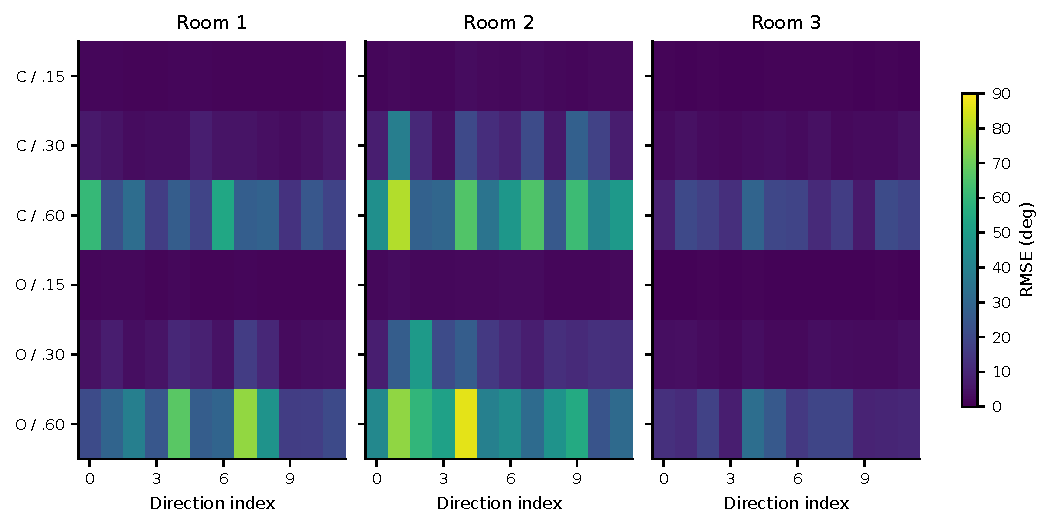
\includegraphics[width=\textwidth]{supp_core_scene_map.pdf}
\caption{Corrected core RMSE at 10 dB, retaining every scene/direction. C/O denote centered/offset array positions; the following number is nominal RT in seconds. Direction index $j$ means $7.37^\circ+30^\circ j$. Large errors remain visible. These 216 cells are fixed acoustic scenes, each with five independent 32-frame recordings.}
\end{figure}

\section{Geometry-only timing bound}
Let $M\in\mathbb R^{3\times2}$ contain centered microphone coordinates and
\begin{equation}
B=\begin{bmatrix}1&-1&0\\1&0&-1\\0&1&-1\end{bmatrix},\qquad A=BM.
\end{equation}
For exact microphone arrival vector $\mathbf t$, $\widetilde{\mathbf u}=-cA^+B\mathbf t$. A perturbation $\boldsymbol\epsilon$ therefore produces the exact vector change $J\boldsymbol\epsilon$, where $J=-cA^+B$. The three pair errors obey a shared-microphone relationship and are not varied independently.

For $|\epsilon_i|\leq h$, the image of the box under $J$ is a convex polygon. If its largest vertex norm $\rho$ is below $\|\widetilde{\mathbf u}\|$, the translated polygon excludes the origin and lies in a common angular half-plane. Along each straight edge the argument is monotone or constant, so angular extrema occur at vertices. Evaluating the eight sign combinations gives the exact worst angular error over the arrival box. The containing disk gives the simpler bound $\arcsin(\rho/\|\widetilde{\mathbf u}\|)$. When the disk condition fails, the implementation returns an uninformative $180^\circ$ bound instead of applying this formula outside its domain.

For an equilateral array of radius $R$, $M^TM=(3R^2/2)I$, $B^TB=3I-\mathbf1\mathbf1^T$, and $\mathbf1^TM=0$. Hence $J=-(2c/3R^2)M^T$. The largest box-vertex sum has magnitude $2hR$, giving $\rho=4ch/(3R)$. For a plane wave, a sufficient timing condition for angular perturbation at most $\eta$ is
\begin{equation}
h\leq\frac{3R}{4c}\sin\eta.
\end{equation}
At $R=5$ cm and $\eta=0.5^\circ$, this is $h\leq0.95407$ microseconds. It is conservative and sufficient, not necessary. A common arrival error cancels through $B$. Finite-distance curvature remains in the unperturbed solution and is not removed by the bound.

For small changes, a unit tangent $\mathbf q$ perpendicular to $\widetilde{\mathbf u}$ gives $\delta\theta\simeq\mathbf q^TJ\boldsymbol\epsilon/\|\widetilde{\mathbf u}\|$. Its box bound is $h\|\mathbf q^TJ\|_1/\|\widetilde{\mathbf u}\|$ in radians. The linear expression can understate finite changes and is not the certification rule. The implementation verifies 34,560 actual rounding cases and 12,000 independent random perturbations across 600 geometries/directions/distances/rates, including non-equilateral arrays. The scalar reference does not import the production solve. Noise, reflected paths, spectral weighting and GCC peak changes lie outside the bound's domain.

\section{Paired contrasts and uncertainty}
For each fixed scene, record and frame, the eight conditions share the same underlying source and noise. Code letters are F/Q (fractional/rounded), S/O (steady/onset), and D/R (direct/reflected). The FSR record in the attribution study is the same input and estimate as its core counterpart. Pairing is checked through input identities and complete frame indices. The core matrix has three SNRs, but attribution and long-record studies use only 10 dB.

For response $z=e$ or $z=e^2$, a rounding main effect is the mean of $z_Q-z_F$ over the four startup/reflection combinations. The onset and reflection effects are analogous. A two-factor interaction is a difference of differences averaged over the remaining factor. With factor codes $x_a\in\{-1,+1\}$, a $k$-factor contrast has coefficient $(2^k/8)\prod_a x_a$ for each of the eight cells. These definitions retain interactions and do not assume additive independent errors.

\begin{table}[htbp]\centering\small
\caption{Factorial squared-error contrasts over the 72 paired scenes. Units are deg$^2$. Positive rounding means Q minus F; onset means O minus S; reflections means R minus D.}
\begin{tabular}{@{}lrrr@{}}\toprule
Contrast & Estimate & Lower 95\% & Upper 95\%\\\midrule
rounding & 19.8190 & 6.6298 & 33.0747\\
onset & -24.5230 & -32.9687 & -15.9631\\
reflections & 741.9518 & 692.9799 & 790.4446\\
rounding $\times$ onset & -6.2482 & -15.1269 & 2.2190\\
rounding $\times$ reflections & 30.7624 & 4.7696 & 57.7907\\
onset $\times$ reflections & -49.0464 & -65.5736 & -32.8908\\
rounding $\times$ onset $\times$ reflections & -12.4964 & -29.9539 & 5.1419\\
\bottomrule\end{tabular}\end{table}


Each contrast is averaged within a complete record before uncertainty is calculated. A bootstrap draw selects five whole records with replacement independently within each scene, uses the same selected records in all paired variants, and averages over the fixed scenes. Two thousand such draws provide percentile intervals. For RMSE, mean squared error is aggregated first and then square-rooted; averaging RMSE values would target a different quantity. Circular bias uses the argument of the mean unit phasor. Bias intervals unwrap bootstrap angles around the reported point estimate.

Medians and 90th percentiles are descriptive point estimates. A $5^\circ$ exceedance rate is retained for each record/scene; this threshold was fixed before the main results. Five independent records per scene give limited within-scene resampling support. No simultaneous-coverage or population-of-rooms claim is made, and the intervals have not been calibrated through a separate statistical simulation.

\section{Averaging and method comparisons}
For each of 72 scenes, training records 0--4 and held-out records 5--9 have distinct source and noise identities. Circular averaging uses nonoverlapping blocks of 1--128 contiguous frames. At 128 frames there is one block per held-out recording, so the pooled high subset contains 180 block estimates, not thousands of independent long-duration observations.

The covariance prediction is a small-error approximation. After centering each training record, lagged products estimate $\gamma_\ell$. Lags above 32 are excluded and retained nonzero lags receive weight $1-\ell/33$. For block length $n$, the sum also receives the finite-average weight $1-\ell/n$. The fitted bias is the pooled training circular mean. An independent-frame comparator uses only $\gamma_0/n$. These are predictions, not bootstrap intervals. The concentration rule is fixed using training data alone: resultant at least 0.95 and absolute mean error at most $15^\circ$. Empirical held-out distributions remain available for every excluded scene. Even an eligible scene can contain rare large errors.

SRP uses the same preprocessed and regularized pair spectra as the GCC front end. For candidate azimuth $\theta$, it maximizes
\begin{equation}
P(\theta)=\sum_{i<j}\Re\sum_{k\in\mathcal B}W_{ij}[k]
 \exp\left(2\pi i f_k\tau_{ij}(\theta)\right),\quad
\tau_{ij}(\theta)=-\frac{(\mathbf m_i-\mathbf m_j)^T\mathbf u(\theta)}{c}.
\end{equation}
The angular grid is periodic, and a three-point quadratic refinement uses wrapped neighboring grid points. Both signs and refinement are checked with independent plane-wave harmonic signals. This score is defined here explicitly; no uninspected performance numbers from another implementation are adopted.

The lower-source-band sensitivity retains the fixed 300--3400 Hz acquisition and estimator bands. Noise above 1700 Hz is therefore present without useful source energy in that part of the band. This is a deliberate robustness probe, not a claim that bandwidth alone explains all differences. Rotation, unequal geometry and unequal wall tests use separately identified random records. Their aggregate contrasts with the base case are not reported as matched causal estimates.

\section{Reproducibility record and release contents}
The local bundle contains the final manuscript and bibliography, vector and raster figures, complete per-frame CSV files compressed with gzip, per-scene metadata, analysis tables, numerical controls, pinned requirements, source code, provenance records and an author-review brief. A manifest records SHA-256 checksums. No historical microphone recordings or publisher full texts are required for the main study. The older analytical diagnostic is included only to reproduce the audit of previous numbers.

A fresh Python environment with the pinned packages reproduced the numerical checks, 8,640 primary estimates in three complete scenes, and the six main PNG figures. The maximum reproduced main-estimate difference was 0 degrees. All other frame identities and failure flags matched exactly. The six main PNG files were byte-identical. The recorded reference runs included the complete direct-path sweep, the joint final duration/domain check, and the independent final room reference. This was a representative reproduction, not another full revised campaign. The complete report is supplied as a machine-readable JSON file.


Full instructions appear in the bundle's reproduction guide. They distinguish reusing retained outputs, rerunning representative records and repeating the full campaign. The number of independent records and exact numerical tolerances are reported rather than describing a representative rerun as a second complete replication. Optional cached impulse responses improve speed but are not needed to regenerate results from configuration and seed identities.

\section{Provenance and exclusions}
The pre-execution workspace was archived and all 1102 archived files were verified against their SHA-256 manifest. The forced 77\% historical illustration, undocumented hardware timing/power claims and unverified measured-localization claims are excluded. Old seven-direction calculations are used only in an explicitly labeled analytical audit, not as end-to-end accuracy evidence.

AI assistance was substantive in planning, mathematics, code, independent reference implementations, literature synthesis, analysis, deterministic scientific plotting and drafting. The human author selected the direction and self-funded the work; final claim review and release approval remain pending. Source reading levels are recorded: bibliographic/abstract checks are not relabeled as full-text reading. The work makes no claim of being the first use of GCC-PHAT, fractional delays, an equilateral microphone array, the image method, or bootstrap uncertainty. The intended contribution is the controlled and reproducible attribution study, with its numerical correction and limitations visible.
\end{document}
